\documentclass[../master.tex]{subfiles}
\begin{document}

Первая задача заключается в математическом моделировании течения несжимаемой жидкости вдоль пластины с малой локализованной в точке $(x_0,z_0)$ неровностью в трехмерном случае.
\begin{figure}[H]
	\begin{center}
		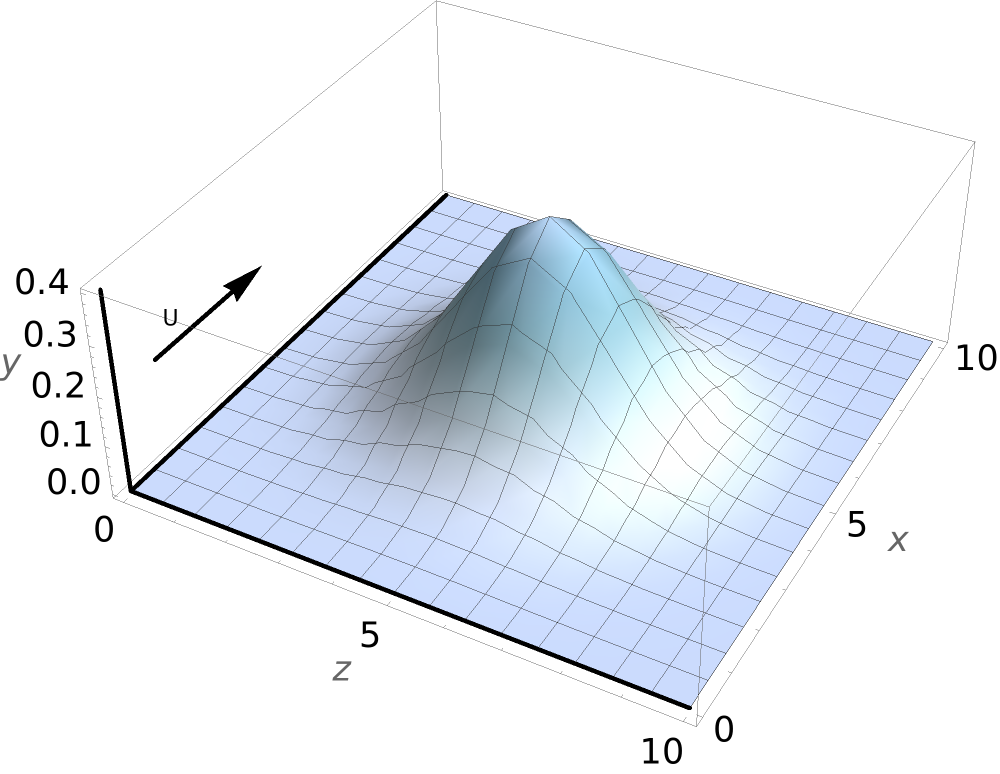
\includegraphics[width=0.6\columnwidth]{3dhump.png}	
		\caption{Обтекаемая поверхность}	
	\end{center}
\end{figure}
Поверхность пластины имеет вид:
\[y_s = \varepsilon^{4/3} \mu\big( (x-x_0)/\varepsilon, (z-z_0)/\varepsilon\big),\]
где $\varepsilon = \mathrm{Re}^{-1/2}$~--- малый параметр, а $\mu$~--- некоторая гладкая функция, убывающая по обоим аргументам на $\pm\infty$.

На пластину набегает плоскопараллельный поток со скоростью $\mathbf u_\infty = (1,0,0)$ и давлением $p_0=\mathrm{const}$. 

Решение такой задачи в случае отсутствия неровности  выражается через функцию Блазиуса~$f(\gamma)$.

\section*{Получение асимптотик решения}
\subfile{math/master}
\section*{Численное моделирование}
\subfile{programming/master}


\end{document}